%%%%%%%%%%%%%%%%%%%%%%%%%%%%%%%%%%%%%%%%%%%%%%%%%%%%%%%%%%%%%%%%%%%%%%%%%%%%%%%%
%2345678901234567890123456789012345678901234567890123456789012345678901234567890
%        1         2         3         4         5         6         7         8

\documentclass[letterpaper, 10 pt, conference]{ieeeconf}  % Comment this line out
                                                          % if you need a4paper
%\documentclass[a4paper, 10pt, conference]{ieeeconf}      % Use this line for a4
                                                          % paper

\IEEEoverridecommandlockouts                              % This command is only
                                                          % needed if you want to
                                                          % use the \thanks command
\overrideIEEEmargins
% See the \addtolength command later in the file to balance the column lengths
% on the last page of the document



% The following packages can be found on http:\\www.ctan.org
\usepackage{graphics} % for pdf, bitmapped graphics files
\usepackage{epsfig} % for postscript graphics files
\usepackage{mathptmx} % assumes new font selection scheme installed
\usepackage{times} % assumes new font selection scheme installed
\usepackage{amsmath} % assumes amsmath package installed
\usepackage{amssymb}  % assumes amsmath package installed
\usepackage{smartdiagram}
\usepackage{tikz}
\usepackage{verbatim}
\usepackage{algorithm2e}




\title{\LARGE \bf
LightGBM: an Effective Decision Tree Gradient Boosting Method to Predict Customer Loyalty in the Finance Industry*
}

%\author{ \parbox{3 in}{\centering Huibert Kwakernaak*
%         \thanks{*Use the $\backslash$thanks command to put information here}\\
%         Faculty of Electrical Engineering, Mathematics and Computer Science\\
%         University of Twente\\
%         7500 AE Enschede, The Netherlands\\
%         {\tt\small h.kwakernaak@autsubmit.com}}
%         \hspace*{ 0.5 in}
%         \parbox{3 in}{ \centering Pradeep Misra**
%         \thanks{**The footnote marks may be inserted manually}\\
%        Department of Electrical Engineering \\
%         Wright State University\\
%         Dayton, OH 45435, USA\\
%         {\tt\small pmisra@cs.wright.edu}}
%}

\author{Marcos Roberto Machado$^{1}$, Salma Karray$^{1}$ % <-this % stops a space
\thanks{*Submitted to Prof. Dra. Salma Karray as a report/article suggestion. This text was elaborated based on a ML grad course presentation performed at The Fields Institute in April 2019.}% <-this % stops a space
\thanks{$^{1}$University of Ontario Institute of Technology}
%,
%        University of Twente, 7500 AE Enschede, The Netherlands
%        {\tt\small h.kwakernaak at papercept.net}}%
%\thanks{$^{2}$P. Misra is with the Department of Electrical Engineering, Wright State University,
%        Dayton, OH 45435, USA
%        {\tt\small p.misra at ieee.org}}%
}




\begin{document}



\maketitle
\thispagestyle{empty}
\pagestyle{empty}


%%%%%%%%%%%%%%%%%%%%%%%%%%%%%%%%%%%%%%%%%%%%%%%%%%%%%%%%%%%%%%%%%%%%%%%%%%%%%%%%
\begin{abstract}
This study presents an implementation of a Machine Learning model, using LightGBM  algorithm, in the financial sector to predict credit card customer loyalty, as a real company's problem. The offer of new algorithm options to be used in different industries have been increasing, and a result new models should be tested and compared with existent ones. This study compares the accuracy of LightGBM, which does not present applications in the financial industry, with XGBoosting, being both Gradient Boosting Decision Trees Models, these article presents the main method used by them. Also, an implementation of LightGB is performed over a Kaggle's competition, where a company aims to classify each customer of their base with a loyalty score for a given set of features. Results are presented, examined and discussed and customer loyalty prediction accuracy is measured through RMSE and compared between LightGBM and XGBoosting.
\end{abstract}


%%%%%%%%%%%%%%%%%%%%%%%%%%%%%%%%%%%%%%%%%%%%%%%%%%%%%%%%%%%%%%%%%%%%%%%%%%%%%%%%
\section{INTRODUCTION}
In order to maximize profits, companies have to invest their efforts in trying to retain customers, boosting customer satisfaction levels and as a consequence escalating their loyalty. The intensity of customers satisfaction is a key metric for a company's CRM (Customer Relationship Management) and as a consequence, loyalty can be measured and analyzed as well. Although customer satisfaction and loyalty are key mediators of profit, they cannot be taken as simple predictors of it. From a business standpoint, it is more important to identify and nurture relationships, specifically with profitable customers (Kumar and Reinartz, 2012 \cite{Kumar2012}). In this context artificial intelligence can be used through the application of Machine Learning (ML) and Deep Learning (DL) models given the extraordinary amount of customer information to businesses available in different sources.\\

ML and DL models can be applied within customer loyalty context from two different point of views. Firstly, it can be used to measure loyalty given customer information, and, secondly, it can be applied to improve the customer satisfaction by providing the right product or service in the right channel/place at the correct time. In both cases, ML/DL models would learn from previous customer interactions. It is so important to be focus on customer satisfaction and loyalty that, according to Gerry Brown from IDC, 2017 \cite{IDC2017}, 65\% of the marketing executives surveyed pointed out that ``real-time personalized advertising insertions" and ``optimized message targeting" will convey a compelling value by 2020. Also, a research published by MIT and Google said that 50\% of businesses intend to apply ML for customers insights, and 48\% expect it to earn a competitive advantage. \\ 

Serkan, 2016 \cite{Loyal2016}; Ajay et al. 2019 \cite{loyal2019} and Davies et al. 2018 \cite{loyal2018} have applied ML in order to study customer loyalty in different settings. More general, other business metrics such as customer lifetime value (CLV), customer retention or customer churn were also explored using ML models and different applications were found in the literature (Jamalian and Foukerdi, 2018 \cite{Jamalian2018}, Jing and Xing-hua, 2008 \cite{Zhao2008}, Amin et al. 2017 \cite{Amin2018} and Amin et al. 2018 \cite{Amin2018}). However, none of these applications studied customer loyalty for credit card customers using LightGBM model.\\

The aim of this study is to explore the application of LightGBM as a predictor for customer loyalty score. The problem was motivated based on an online competition (Kaggle, \cite{Kaggle}), where a credit card company was looking for a ML model that make prediction of customer loyalty score for each single Card ID (for each single card issued) possible. Company was also requesting a RMSE (Root Mean Square Error) to be presented along to the loyalty score predicted. These type of problem is getting more and more common in the financial industry, where, with more customer data it is more important to anticipate customers needs in order to retain them, increasing their loyalty. LightGBM as applied as the main ML method, mainly based on its capacity to uses GPU and uses less memory, the possibility to get high speed and handle large size of data. Also, because it present better accuracy than other decision tree gradient boosting models such as XGBoosting (Ke et al., 2017 \cite{LGBM}) and by reason of its application was not found at the CRM/Loyalty literature.

\section{LITERATURE REVIEW}
\subsection{Decision Tree Models}
One of the most common classification technique is the Decision Tree (Seni and Elder, 2010 \cite{Seni2010}). Figure \ref{DT}, presents a flowchart, which exemplifies a decision tree. It is composed of decision blocks (rectangles) and terminating blocks (circles), which present the conclusion or final classification. Arrows in the flowchart represent branches that can lead to decision blocks or terminating blocks (Harrington, 2012 \cite{Harrington2012}). In this example, a decision between approval or denial of a credit card is build, where income and credit score are features or variables that will decide final classification.\\

\tikzstyle{box} = [rectangle, rounded corners, minimum width=3cm, minimum height=1cm,text centered, draw=black, fill=blue!30]

\tikzstyle{circ} = [circle, minimum width=1.5cm, text centered, draw=black, fill=red!30]

\begin{figure}[thpb]
\begin{center}
\begin{tikzpicture}
\begin{small}
\node (Credit Card Approval) [box] {Credit Card Approval};
\node (yes) [circ, below of=Credit Card Approval, yshift=-1.5cm] {Declined };
\node (hum) [circ, left of=yes, xshift=-1.2cm] {Approved};
\node (wind) [box, right of=yes, xshift=1.6cm] {Credit Score Analysis};

\draw [->] (Credit Card Approval) -- (yes) node[pos=0.3, right] {Income $<500$};
\draw [->] (Credit Card Approval) -- (hum) node[pos=0.5, left] {Income $>1,000$};
\draw [->] (Credit Card Approval) -- (wind) node[pos=0.6, right] {$500<\text{Income}<1,000$};

\node (yes2) [circ, below of=wind, yshift=-1.2cm, xshift=1.1cm] {Declined};
\node (no2) [circ, below of=wind, yshift=-1.2cm, xshift=-1.1cm] {Approved};

\draw [->] (wind) -- (yes2) node[midway, right] {Bad Score};
\draw [->] (wind) -- (no2) node[midway, left] {Good Score};

\end{small}
\end{tikzpicture}
\end{center}
\caption{Decision Tree example. A decision over issue customer with a credit card or not can be performed following this model, where customer income and credit score are features analyzed to make a decision.}
\label{DT}
\end{figure}

Decision tree models are computationally cheap to use, easy for humans to understand learned results, handle missing value/information well, can deal with irrelevant features, works with numerical and nominal values, however, it tends to overfit (Bishop, 2006 \cite{Bishop2006} and Russell and Norvig, 2009 \cite{Russell_Norvig2009}). Another important concept with respect to these type of models is split. It is necessary to choose which feature will be choosen to split the data in order to guarantee the best results possible. The decision on how to split data should be performed the same way repeatedly until all data has been classified. Data split in decision tree models had been performed using different measures in different studies (Dietterich, 2000 \cite{Dietterich2000}, Kohavi et al., 2002 \cite{Kohavi_etall2002}, Quinlan, 1986 \cite{Quinlan1986} and Fayyad and Irani, 1992 \cite{Fayyad_Irani1992}). Moreover, the most common metrics are the Gini Impurity, Information Gain (Entropy) and Variance Reduction (Harrington, 2012 \cite{Harrington2012} and Russell and Norvig, 2009 \cite{Russell_Norvig2009}). Variance reduction of Gain of Variance is the metric used in XGBoosting and LightGBM, which will be explored in detail in this study.

\subsection{Gradient Boosting Models}

Another machine learning technique used for regression and classification is gradient boosting. The output of the models built with the application of this technique does perform a prediction in the form of an ensemble of weak prediction models, decision trees (Bishop, 2006 \cite{Bishop2006} and Harrington, 2012 \cite{Harrington2012}). Leo Breiman (\cite{Breiman97}) first presented the idea that boosting can be interpreted as an optimization algorithm for a given cost function. Later on, regressions gradient boosting algorithms were implemented by different authors (Friedman, 1999 \cite{Friedman2000}, Friedman, 2000 \cite{Friedman2000} and Elith et al., 2008 \cite{Elith2008}) using a different and practical viewpoint (Mason et al., 1999 \cite{Mason99} and Mason et al., 2000 \cite{Mason00}). As a consequence, the development of different boosting algorithms in different areas such as Statistics and AI (Artificial Intelligence) is observed (Grabner and Bischof, 2006 \cite{Grabner2006}, Lee et al., 2010 \cite{Lee2010} and Shabtai et al., 2009 \cite{SHABTAI2009}).\\

In order to perform predictions, gradient boosting uses a strong learner -- a classifier arbitrarily well-correlated with the true classification -- which is build from the combination of different weak learners -- classifiers that are only slightly correlated with the true classification -- this approach is applied in a iterative method (Li, 2017 \cite{Li__2017}).\\

For the gradient boosting algorithm, as in any other machine learning supervised problem, there is a vector of features $x$ that will be used to predict an output variable $y$ through a probability distribution $P(x,y)$. Thus, a data set  $\{(x_i,y_i)\}_{i=1}^n$ is needed and the aim of the algorithm is to find an approximation $\hat{F}(x)$ to a function $F(x)$ which will minimize the value of a certain loss function $L(y_i,F(x))$. Thus, assuming a value $y$, the gradient boosting algorithm will look for an approximation $\hat{F}(x)$ in the form of a weighted sum of functions, from different classes of (weak) learners.\\

Algorithm 1 presents the pseudo-code on how the gradient boosting algorithm works. For a given data set, $\{(x_i,y_i)\}_{i=1}^n$, and lost function, $L(y_i,F(x_i))$, the procedure initiate assuming a constant as the predictor that minimize the loss function. Then, in the step 2, the residuals $(r_{im})$ are calculated for each observation $m$ in the data set (which, will logically provide the gradient boosting calculation), then a regression is fitted over the residuals calculation creating terminal regions $(R_{jm})$ for possible classifications, after that, the minimum value of each terminal $(\gamma_{jm})$, that were already defined is verified (which is the average in each region defined), and finally the constant (average) with which the iteration process started will be optimize in each integration time step in order to perform the final prediction $(F_m(x))$.

\begin{algorithm}
\SetAlgoLined
\textbf{Input:} Data $\{(x_i,y_i)\}_{i=1}^n$, and a differentiable loss function $L(y_i,F(x_i))$.\\	
\textbf{Step 1:} Initialize model with a constant: $F_0(x)=\underset{\gamma}{\min}\sum_{i=1}^nL(y_i,\gamma)$.\\
\textbf{Step 2:} for $m=1$ to $M$:
\begin{itemize}
\item Compute $r_{im}=-\left[\frac{\partial L(y_i,F(x_i))}{\partial F(x_i)}\right]_{F(x)=F_{m-1}(x)}$ for $i=1,2,...,n$; 
\item Fit a regression tree to the $r_{im}$ values and create terminal regions $R_{jm}$ for $j=1,2...,J_m$ ;
\item For $j=1,2,..., J_m$ compute $\gamma_{jm}=\underset{\gamma}{\min} \sum_{x_i\in R_{ij}}L(y_i,F_{m-1}(x_i)+\gamma)$ ;
\item Update $F_m(x)=F_{m-1}(x)+\nu \sum_{j=1}^{J_m} \gamma_{jm} I(x \in R_{jm})$;
\end{itemize}
\textbf{Step 3:} Output $F_m(x)$.\\~\\
\caption{Gradient Boosting Algorithm -- Pseudo Code (Source: Scikit Learn, 2019 \cite{scikitlearn_2019}, adapted by the author).}
\end{algorithm}

\subsection{GBDT Models}
Gradient Boosting Decision Tree (GBDT) models combine the two techniques already presented in this study, usually through decision tree models, for instance XGBoosting, which is one of the most used GBDT algorithms (Torlay, 2017 \cite{Torlay2017}, Zheng et al., 2017 \cite{Zheng2017} and Chen and Guestrin, 2016 \cite{ChenGuestrin2016}).\\

These models are characterized mainly by the way that the splits are performed when the trees are growing in the processes. Most of the GBDT models, like XGBoosting, does perform splits by calculating the Gain of Variance (Equation 1). For instance, letting $O$ be the training set on a fixed node of the decision tree. The variance gain of splitting feature $j$ at point $d$ for this node is presented in Equation 1 (Ke at al., 2017 \cite{LGBM}).

\begin{equation}
V_{j\mid O}(d)=\frac{1}{n_{O}}\left(\frac{\left(\sum_{x_{i}\in O:x_{ij}\leqslant d} g_{i}\right)^{2} }{n_{l\mid O}^{j}(d)}+\frac{\left(\sum_{x_{i}\in O:x_{ij}>  d} g_{i}\right)^{2}  }{n_{r\mid O}^{j}(d)}\right)
\end{equation}
where
$g_i$ is the negative gradient of the loss function with respect to the output of the model, $n_{O}=\sum I[x_{i} \in O]$ which is the total number of observations in the data set $O$, $n_{l\mid O}^{j}(d)=\sum I[x_{i} \in O:x_{ij}\leqslant d]$ is the total number of observations  at the left of the data set and $n_{r\mid O}^{j}(d)=\sum I[x_{i} \in O:x_{ij} >d]$ is the total number of observations  at the right of the data set. For a feature $j$, the decision tree algorithm selects $d_{j}^{*}=argmax_{d}V_{j}(d)$ and calculate the largest gain $V_{j}(d_{j}^{*})$. Then, the data are split according feature $j^{*}$ at the point $d_{j^{*}}$ into the left and right child nodes.\\

Most decision tree learning algorithms, such as XGBoosting, grow trees by level (depth), which means that at each integration time step, all nodes in the deepest level grow (Figure \ref{level_wise_tree}).

\begin{figure}[thpb]
\centering
%\framebox{\parbox{3in}{We suggest that you use a text box to insert a graphic (which is ideally a 300 dpi TIFF or EPS file, with all fonts embedded) because, in an document, this method is somewhat more stable than directly inserting a picture.
%}}
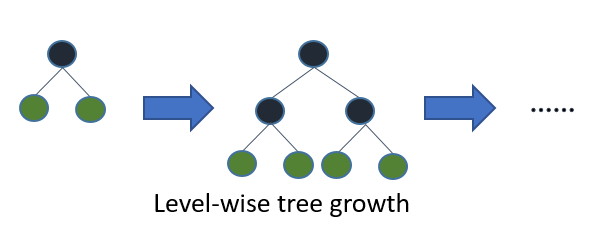
\includegraphics[scale=0.5]{Figures/level-wise.png}
\caption{GBDT Models - Growing tree level-wise within model training, all nodes grow in each iteration (Source: LightGBM Documentation, 2019 \cite{LightGBM2019}).}
\label{level_wise_tree}
\end{figure}


\subsubsection{LightGBM}
LightGBM is an open source GBDT algorithm by Microsoft. It uses a histogram-based algorithm (Alsabti et al., 1999 \cite{Alsabti1999}) to speed up the training process, reduce memory consumption and combines advanced network communication to optimize parallel learning, called parallel voting decision tree algorithm (Wang et al., 2017 \cite{Wang2017} and Ke at al., 2017 \cite{LGBM}). Also,  LightGBM uses the leaf-wise strategy to grow trees and to find a leaf with largest gain of variance to do the split (Figure \ref{leaf_wise_tree}).\\

LightGBM can be differentiated from other GBDT models by the way the gain of variation is calculated (Equation 2). Considering the same inputs presented for the calculation of the gain of variance in Equation 1, in lightGBM, the splits occur considering weak and strong learners (small and big gradients $(g_i)$. In this case, the training instances are rank according to the absolute values of their gradients in the descending order; then, a top $a$ percent of instances with the larger gradients are kept to form an instance subset $A$. Then, for the remaining set $A^c$ formed by the $(1 - a)$ percent of instances with smaller gradients, a subset $B$ with size $b \times |A^c|$ is randomly formed; finally, the split of the instances according to a estimated variance gain $V^*_j(d)$ over the subset $A \cup B$ is performed (Equation 2, Ke at al., 2017 \cite{LGBM}).

\begin{equation}
\begin{split}
V^*_j(d)=\frac{1}{n}\left(\frac{\left(\sum_{x_i\in A_l} g_i+ \frac{1-a}{b} \sum_{x_i\in B_l} g_i\right)^2 }{n_l^j(d)}  \right. \\
\left. +\frac{\left(\sum_{x_i\in A_r} g_i+ \frac{1-a}{b} \sum_{x_i\in B_r}g_i\right)^2}{n_r^j(d)}\right)
\end{split}
\end{equation}
where $A_l=\{x_i \in A: x_{ij} \leqslant d\}$, $A_r=\{x_i \in A: x_{ij} > d\}$, $B_l=\{x_i \in B: x_{ij} \leqslant d\}$, $B_r=\{x_i \in B: x_{ij} > d\}$, where $d$ is the point in data where the split is calculated in order to find the optimal gain in variance, and the coefficient $\frac{1-a}{b}$ is used to normalize the sum of the gradients over B back to the size of $A^c$.\\


\begin{figure}[thpb]
\centering
%\framebox{\parbox{3in}{We suggest that you use a text box to insert a graphic (which is ideally a 300 dpi TIFF or EPS file, with all fonts embedded) because, in an document, this method is somewhat more stable than directly inserting a picture.
%}}
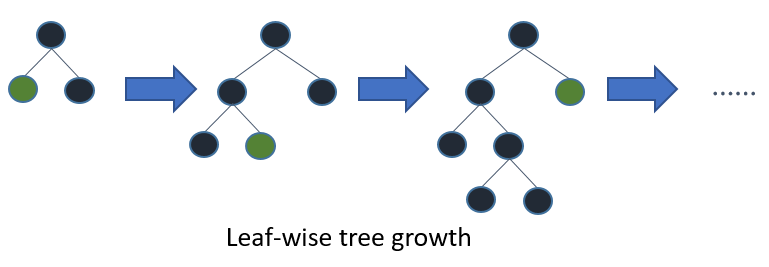
\includegraphics[scale=0.4]{Figures/leaf-wise.png}
\caption{LightGBM - Growing tree leaf-wise within model training, not all nodes grow in each integration time step, just the node that present optimal gain of variance is choose to grow and split (Source: LightGBM Documentation, 2019 \cite{LightGBM2019}).}
\label{leaf_wise_tree}
\end{figure}

The gain of variance methodology, including the consideration of weak learners within the algorithms and the methodology to grow trees combined make LightGBM offer a better classification/prediction than other GBDT models (Ke at al., 2017 \cite{LGBM}). Applications of LightGBM algorithm can be found in the literature in different industries to deal with different problems (Wang et al., 2017 \cite{Wang2017}, Sun et al., 2018 \cite{SUN2018} and Ma et al., 2018 \cite{MA201824}). However, because none of the applications of this algorithm were found in Business, Marketing of Financial setting, this study aims to compare its applicability, performance and accuracy when compared with another standard GBDT model (XGBoosting).


\section{METHODOLOGY}
\subsection{Datasets}

Elo is one of the largest payment brands in South America. Elo results from a partnership of three of the largest banks in Brazil: Banco do Brasil, Bradesco and CAIXA. Elo offers credit, debit, and prepaid cards. At the end of 2018, Elo had issued more than 50 million cards. Also, Elo credit card supports installment payments, which allows a customer to arrange payments over a period of time (Kaggle / Elo, 2018 \cite{Kaggle}) .\\

Elo has built partnerships with merchants in order to offer promotions or discounts to cardholders. They have built machine learning models to understand the most important aspects and preferences in their customers’ lifecycle, from food to shopping. They have also built machine learning models to attribute a loyalty score for cluster of customers (per segment), however so far none of them is specifically tailored for an individual or profile (Kaggle / Elo, 2018 \cite{Kaggle}). This is where the Kaggle competition and data made available comes in. The main objective is to develop algorithms to identify customer loyalty score for each card identified from the data sets.\\

Different data sets were made available (Figure \ref{Fig_data}). The historical data set has transaction information, features such as purchase date and amount, number of installments, city and state, merchant identification and a sub sector identification of the merchant where card was used. The merchant data set has additional information with respect to the places where cards were used. Features such as merchant identification group, average sales, average purchase, active month lags (amount of months in which card had not being used), city and state of the merchant location were available. New merchant data set has same type of information that historical data frame has, however this set of data contains material info of merchants visited for the first time. Training data set contains the first month of activation, the target (loyalty score) and other features. All five data sets also have anonymous information/features.\\

\begin{figure}[thpb]
\centering
\smartdiagramset{set color list={green!40,magenta!40,blue!50,teal!40,orange!40},uniform connection color=true}
\smartdiagram[descriptive diagram]{
  {Historical,{Up to 3 months of historical transactions for each card identified.}},
  {Merchant, {Additional information about all merchants.}},
  {New Merchant, Two months of data for each card identified containing all purchases from each card made at each merchant not visited in the historical data.},
  {Test, The test set - which contains different features from the historical data.},
  {Train, The training set in the same format of the test set dataset.}}
\caption{Five different datasets were made available from ELO, a credit card company. Dataset are briefly described, each dataframe has different set of infromations. Data was published at kaggle.com in 2018 \cite{Kaggle}}
\label{Fig_data}
\end{figure}


\subsection{Data Preparation}
Almost all ML algorithms can not perform well with missing values. This was the very first point explored at the Data Preprocessing Treatment (DPT), which is part of what we are calling Data Cleaning. At this stage, for all data sets missing values were replaced based on the following rule: if the number of missing observations were less than 5\% of the total of instances for that feature, those observations were drop, in the other case, the missing value was replaced by the mode of that feature. In addition, an analysis over possible outliers was performed. It is important to highlight that, mainly for the target, 1.1\% (2,207) observations were possible outliers, and given the relevance of the feature in the data, those values were marked, considering the inclusion of a dummy feature in order to identify those.\\

In the second stage of DPT, categorical features were converted to numerical values in order to facilitate things later on in the pipeline process. Codes were attributed to different nominal observation and this standard was applied for all data sets. Then, feature engineering was performed. Firstly, all the data sets were unified/appended by the card identification, then more features were created based on the ones that the company made available. Feature transformers were applied in order to provide more data information for the models to learn better and predict information with higher accuracy. In the fourth stage, a correlation analysis over the features was implemented. When correlation between features and target was higher than 90\%, features (new features created or previous ones) were drooped from the data sets. Finally, at the end of the workflow, a pipeline was implemented in order to select possible models and techniques to be used to train the data and make predictions. A workflow process is presented in Figure \ref{workflow}, where the bottom to top Data Preprocessing Treatment (DPT) performed in this study has been presented. \\


\begin{figure}[thpb]
\centering
\smartdiagramset{set color list={orange!40,teal!40,blue!50,magenta!40,green!40},uniform connection color=true}
\smartdiagram[priority descriptive diagram]{
  Data Cleaning,
  Handling Text and Categorical Attributes,
  Feature Engineering,
  Correlation Analysis,
  Pipe Line Planning}
\caption{Workflow from bottom to top of the Data Preprocessing Treatment (DPT) performed in the datasets in this study. All steps in this process was recommended by Geron, 2017 \cite{Geron} and it is usually performed in an end-to-end ML modelling project.}
\label{workflow}
\end{figure}  
  

\subsection{Model Training}
In order to perform predictions on the test set, the main parameters used in LightGBM training process were:

\begin{itemize}
\item Number of leaves: 31;
\item Minimum amount of data in a leaf: 30;
\item Objective: Regression;
\item Number of threads: 4;
\item Boosting: GBDT
\end{itemize}

Another important thing to mention with respect to the training process is that stratified random sampling method was used in this step. This is a method of sampling that was used to divide the data set that went through the DPT into smaller groups known as strata. In a stratified random sampling method, the strata are formed based on similar attributes or characteristics. Each new sample has the same size. In LightGBM, it is necessary to define the number of strata, which in this study is 5 for all training performed. By using stratified random sampling method, it is possible to have a higher number of subsets to train the model and by doing this we give the model a chance to obtain a better performance, because in this case, each new subset is used once as a test set while the others are used as training ones, until all folders be a test set at least once. 

%	Highlight colors and text:
%	\colorbox{red}{Your first option of version control!!!}
%	\textcolor{blue}{The second option right away!!!!!!!!!}

\subsection{Evaluation Criteria}

Among of all possible metrics, such as Absolute Error, Mean Absolute Error, Mean Squared Error, and Root Mean Squared Error (RMSE), RMSE was used to measure the differences between values predicted by LightGBM and XGboosting. These differences are called residuals and the RMSE is used to track the size of the errors in predictions and measure how well the model perform. Thus, RMSE is a measure of accuracy, to compare forecasting errors of different models for a particular dataset and not between datasets, as it is scale-dependent ((Harrington, 2012 \cite{Harrington2012} and Hyndman and Koehler, 2006 \cite{Hyndman_Koehler2006}).\\

According to Hyndman and Koehler, 2006 \cite{Hyndman_Koehler2006} RMSE is a quadratic scoring rule that measures the average magnitude of the error. It’s the square root of the average of squared differences between prediction and actual observation:

\begin{equation}
RMSE=\sqrt{\frac{1}{n}\sum_{j=1}^n\left(y_j-\hat{y}_j\right)^2}
\end{equation}
where $n$ is the number of observations, $y_j$ are the predicted values and $\hat{y}_j$ are the actual values.\\

As a consequence of Equation 3, RMSE is always non-negative, and a $RMSE=0$ would indicate that the model fits the data set of the problem perfectly, which will never happen. Usually, researches aim to find the minimum RMSE, as it happens in this study.\\

\section{RESULTS}
This section presents how well LightGBM predicted customer loyalty in the financial sector, specifically for the case of Elo credit card company. RMSE has been analyzed altering some of the parameters within the ML training algorithm such as learning rate and number of iterations. Also, a comparison between LightGBM and XGboosting has been performed.

\subsection{RMSE vs Learning Rate}
The model was trained for different learning rates (0.001, 0.005, 0.01, 0.02, 0.03, 0.04, 0.05, 0.06, 0.07, 0.08, 0.09, 0.1) and the RMSE for the predicted loyalty score was calculated. Figure \ref{learning_rate} shows these results. It is possible to verify that when learning rate is approaching zero RMSE is not one of the best results. This happens because given a poor learning rate, when the algorithm is looking for the best solution, a local minimum is found and it is interpreted to be the global minimum. On the other hand, when learning rate is increasing, after a certain point (around learning rate equals to 0.04), the RMSE is no-optimal as well. This behavior is given by the reason of big learning  rates lead makes the algorithm surpass the global minimum, finding at the end a local minimum. For this specific study, a learning rate of 0.01 is optimal, it offers a low RMSE as well as best loyalty score prediction.

\begin{figure}[thpb]
\centering
%\framebox{\parbox{3in}{We suggest that you use a text box to insert a graphic (which is ideally a 300 dpi TIFF or EPS file, with all fonts embedded) because, in an document, this method is somewhat more stable than directly inserting a picture.
%}}
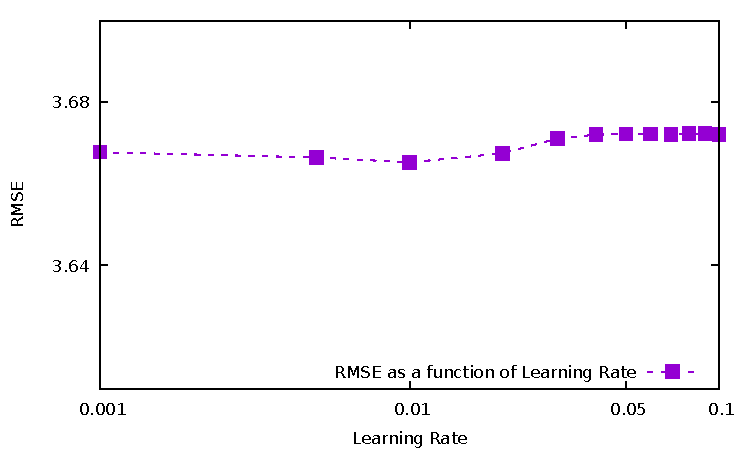
\includegraphics[scale=0.7]{Figures/learningrate_rmse_lgbm.pdf}
\caption{LightGBM results: RMSE as a function of learning rate.}
\label{learning_rate}
\end{figure}


\subsection{RMSE vs Number of Iterations}
For a fixed learning rate of 0.01, which provides the better RMSE as presented previously, different number of iterations was input during model training. Mainly because LightGBM has a Decision Tree model growing in its code, it is important to verify how the RMSE would behave for different number of iterations, mainly because in a decision tree model depending on the number of iterations the model will end it up with a different tree and as a consequence a different prediction. In this setting, different number of iterations were considered and RMSE measured, results are presented in Figure \ref{number_iterations}. \\

Figure \ref{number_iterations} shows that for a small number of iterations, the model does not have time enough time to learn and find best solution and as a consequence a higher RMSE is observed. As the number of iterations increase, the RMSE decreases, up to a certain point where it does not matter how much more the number of iterations increases, the RMSE will not present a significant change, it will just increase the processing time. Therefore, it is plausible to choose between 900-1000 iterations in this study and guarantee the lower RMSE of the series.

\begin{figure}[thpb]
\centering
%\framebox{\parbox{3in}{We suggest that you use a text box to insert a graphic (which is ideally a 300 dpi TIFF or EPS file, with all fonts embedded) because, in an document, this method is somewhat more stable than directly inserting a picture.
%}}
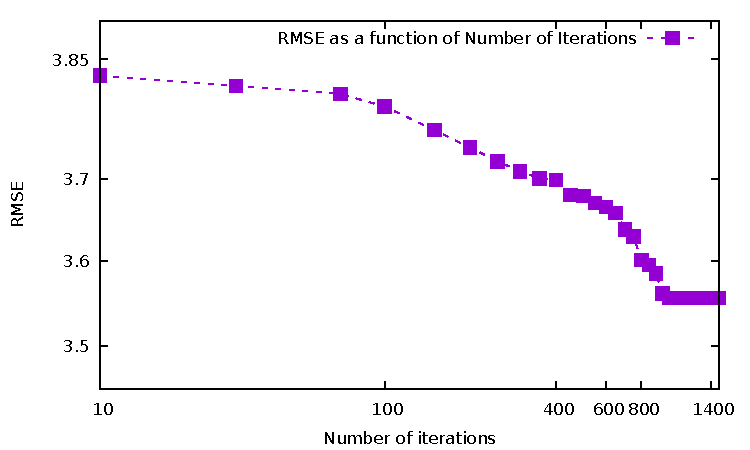
\includegraphics[scale=0.7]{Figures/numinteractions_rmse_lgbm.pdf}
\caption{LightGBM results: RMSE as a function of number of iterations.}
\label{number_iterations}
\end{figure}


\subsection{Training Time}
Another important thing to decide, from the point of view of a prediction model, is based on a trade-off: time versus accuracy. The number of iterations was fixed at 1000 and output measures such as time and RMSE were calculated (Figure \ref{time}). It is possible to observe that for small learning rate time is between the highest in the interval and the RMSE is not optimal, and as the learning rate increases the processing time decreases, however, the RMSE does not show a significant absolute difference in its value. Therefore, depending on the application the CRM will have to decide what is the primary focus - time or accuracy.

\begin{figure}[thpb]
\centering
%\framebox{\parbox{3in}{We suggest that you use a text box to insert a graphic (which is ideally a 300 dpi TIFF or EPS file, with all fonts embedded) because, in an document, this method is somewhat more stable than directly inserting a picture.
%}}
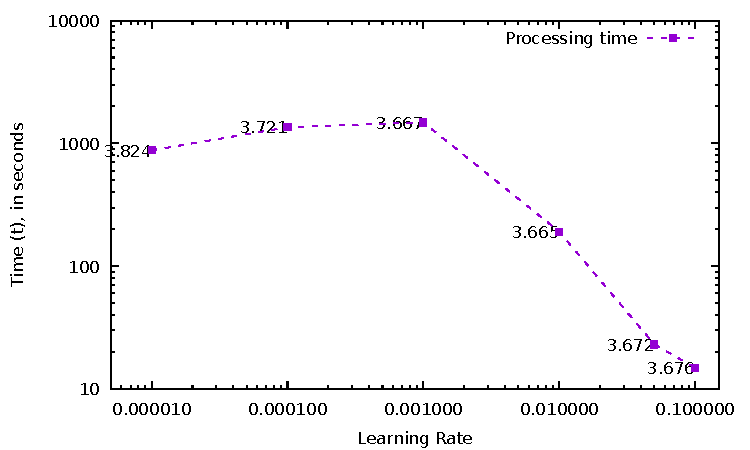
\includegraphics[scale=0.7]{Figures/time.pdf}
\caption{LightGBM results: Time and RMSE as a function of learning rate. RMSE is presented as a label for each point on the dotted line.}
\label{time}
\end{figure}


\subsection{Feature Importance}
Before performing model training, we ended up with more than 230 features. Feature importance in predicting customer loyalty is given through the LightGBM model. Importance of each feature is calculated based on how many times a feature was used to slip information (was used as a node) during the tree growing in the modelling process. Figure \ref{feature_importance} presents the top 8 most important features and the least important to predict customer loyalty in this study, feature importance measure and standard deviation are presented. From approximately 200 features, only as the ones that do not change when the number of iterations or learning rate were altered are presented. It is possible to observe that Month lag Mean, which is the average of months that a card identified was not used is the feature most used to split data in the decision tree process and the Month lag Minimum was the least used one. Standard deviation slightly decreases as the feature importance decreases.

\begin{figure}[thpb]
\centering
%\framebox{\parbox{3in}{We suggest that you use a text box to insert a graphic (which is ideally a 300 dpi TIFF or EPS file, with all fonts embedded) because, in an document, this method is somewhat more stable than directly inserting a picture.
%}}
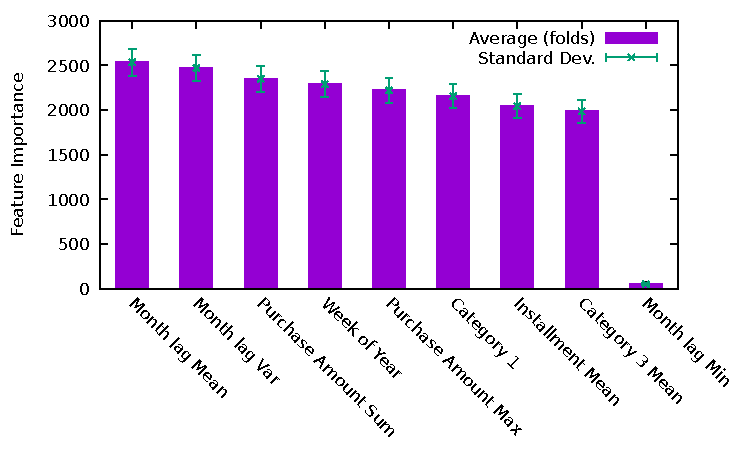
\includegraphics[scale=0.7]{Figures/Feature.pdf}
\caption{LightGBM results: Feature Importance.}
\label{feature_importance}
\end{figure}

\subsection{LightGBM vs XGBoosting}
LightGBM and XGBoosting are based on Decision Tree and Gradient Boosting (DTGB) techniques. However, this section aims to verify Ke et al., 2017 \cite{LGBM} affirmation that LightGBM performs better than XGboosting as a DTGB combined model. Same set of parameters were set up for both scenarios, information such as learning rate and number of iterations were fixed and RMSE was measured for both cases and results are presented in Figure \ref{Xboosting}. It is possible to verify that, for this study, LightGBM perform better than XGBoosting for all interval of learning rate used. Therefore, it is plausible to affirm that LightGBM can also be used as a DTGB model in the financial sector to predict customer loyalty.

\begin{figure}[thpb]
\centering
%\framebox{\parbox{3in}{We suggest that you use a text box to insert a graphic (which is ideally a 300 dpi TIFF or EPS file, with all fonts embedded) because, in an document, this method is somewhat more stable than directly inserting a picture.
%}}
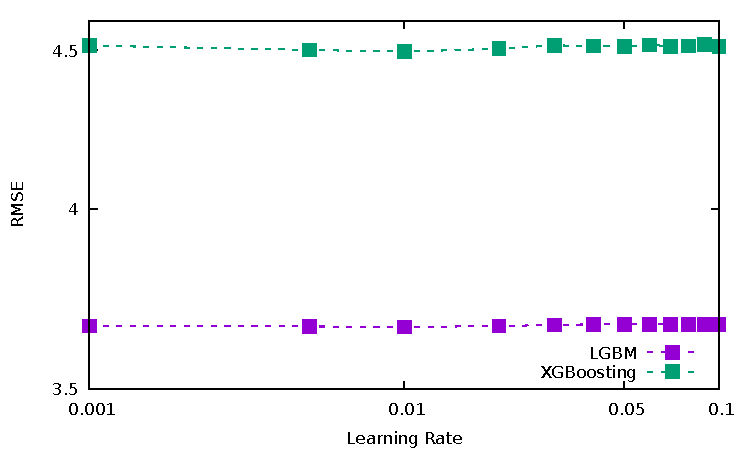
\includegraphics[scale=0.7]{Figures/learningrate_rmse_lgbm2.pdf}
\caption{LightGBM vs XGBoosting: RMSE for customer loyalty prediction.}
\label{Xboosting}
\end{figure}


\section{CONCLUSION}
In this study, LightGBM ML algorithm was applied in a financial setting in order to perform credit card customers loyalty score predictions. We proposed a GBDT model application in this setting, considering that in the literature this model does not appear to be applied exhaustively, specially in the Business/Financial industry. This paper aimed to verify if the accuracy of this model would be better than other types of GBDT algorithm, then a comparison between LightGBM and XGBoosting was also provided.\\

It is possible to verify from the results that, by utilizing a combination of good and weak learners (gradients) in order to look for a global minimum -- which result as the best predictor for the problem, LightGBM does present good results, also when it is compared with XGBoosting.\\

The findings presented in this paper validate the usage of a relatively new GBDT model to be widely applied in the financial sector, once that it presents results with slightly better accuracy than usual regression and other GBDT models.\\

For future studies, comparisons with other type of ML models can be performed, also analyzing the feature importance and training the model with most important features (small number of variables) can boost management strategies in the business, results can be measured and loyalty programs can be developed or enforced based on the customer loyalty prediction performed over this study.


\addtolength{\textheight}{-12cm}   % This command serves to balance the column lengths
                                  % on the last page of the document manually. It shortens
                                  % the textheight of the last page by a suitable amount.
                                  % This command does not take effect until the next page
                                  % so it should come on the page before the last. Make
                                  % sure that you do not shorten the textheight too much.

%%%%%%%%%%%%%%%%%%%%%%%%%%%%%%%%%%%%%%%%%%%%%%%%%%%%%%%%%%%%%%%%%%%%%%%%%%%%%%%%


\bibliographystyle{IEEEtran}
\bibliography{ref.bib}


\end{document}
